
\chapter{Salicórnia: caracterização, importância e cultivo}

A palavra salicórnia deriva do latim tardio \textit{sal}, que significa sal, e \textit{cornus} que significa corno. Etimologicamente a palavra salicórnia significa cornos salgados\cite{chambers}. A espécie de salicórnia que que servirá de mote à elaboração desta dissertação é a única existente em Portugal designada por \sr \textit{J. Woods (S. ramosissima)}\cite{JoaoSilva}, uma espécie do género \textit{Salicornia L.}, pertencente à família das beterrabas denominada de \textit{Chenopodiaceae} \cite{chenopodiaceae}.

Nesta secção será apresentada a \sr que impulsionará toda esta dissertação. Serão descritas as principais características desta planta, principais propriedades e as diferentes aplicações alimentais existentes no mercado. 

\section{Características da planta}


A salicórnia é uma espécie halófita, ou seja adaptada a viver em ambientes com elevado teor salino\cite{ferri}, sendo uma das mais evoluídas da sua família. É uma planta anual de dimensão pequena, aparentemente sem folhas, ereta, os seus caules são carnudos e suculentos, simples e/ou extremamente ramificados, segmentados por articulações\cite{Silva2000}, geralmente com menos de 30 cm de altura\cite{overviewsal}.

A salicórnia tem uma coloração normalmente verde-escuro mas a sua ramagem torna-se  verde-amarelado ou mesmo vermelho-púrpura no outono\cite{Silva2000}. A figura \ref{primoutono} ilustra a respetiva coloração na primavera e no outono. Na Inglaterra, a salicórnia é conhecida como \textit{purple glasswort}, podendo este nome estar na origem desta pigmentação caraterística\cite{Davy2001}. Em Portugal e Espanha é conhecida vulgarmente como erva-salada, sal verde e/ou espargos do mar\cite{RaquelPinto}. 

\newpage
\begin{figure}[!htb]
	\centering
	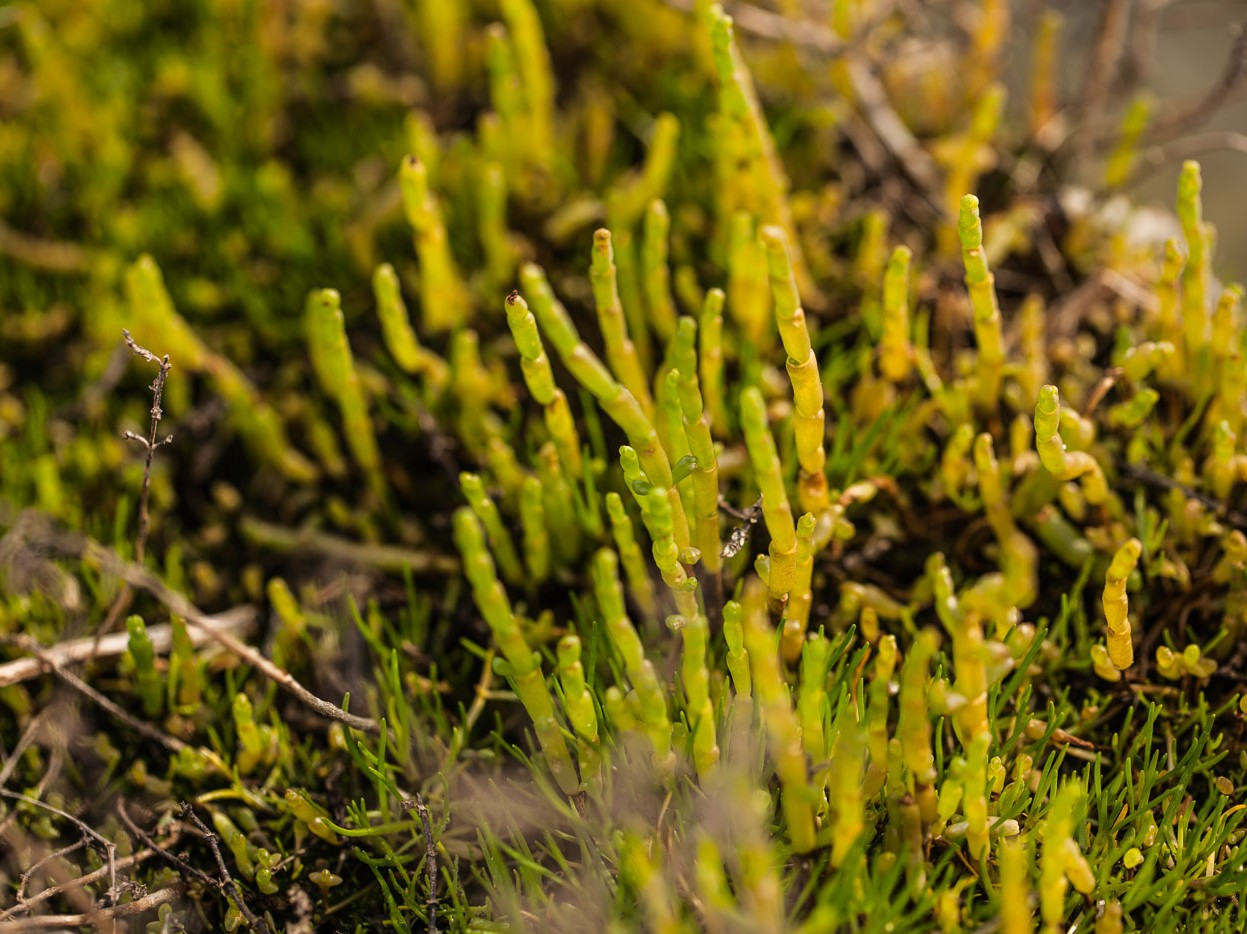
\includegraphics[scale=0.3]{img/cap2-sali/Salicornia04.JPG}
	\caption{\sr: na primavera e no outono respetivamente à esquerda e à direita (Fotografia por José M. G. Pereira)}
	\label{primoutono}
\end{figure}


A \sr desenvolve-se preferencialmente no litoral costeiro, em pântanos e sapais salgados ou em margens de salinas temporariamente alagadas. Encontra-se distribuída maioritariamente na parte oeste da Europa e a oeste da região do Mediterrâneo, sendo uma das espécies mais abundante\cite{Figueroa1987}. Pode ser encontrada em todo o litoral da Península Ibérica, embora com menos frequência no Minho\cite{Silva2000}. Em Portugal, é encontrada ao longo da costa, mais frequentemente nas margens dos canais da Ria de Aveiro e Ria Formosa, no Algarve\cite{RaquelPinto}. 

Esta planta é uma das mais estudadas a nível mundial\cite{Figueroa1987}, possuindo um ciclo de vida anual bem definido, com gerações discretas e as suas sementes são hermafroditas\cite{Silva2007}. A salicórnia cresce habitualmente entre março, início da sementeira e novembro fechando assim o ciclo com a produção de sementes. Entre maio  e agosto decorre a colheita da planta\cite{RaquelPinto} utilizada para os mais diversos fins. A floração ocorre fundamentalmente no mês de outubro\cite{Figueroa1987}. A figura \ref{ciclodevida} representa evolução do estado da planta para as diferentes fases do seu ciclo de vida. 




 \begin{figure}[!htb]
 	\centering
 	
\includegraphics{uaLogoNew.pdf}
 	\caption{Ciclo de vida da \sr (Fotografia por José M. G. Pereira)}
 	\label{ciclodevida}
 \end{figure}
 
 



\newpage

\section{Importância da planta}


Uma das características que tornam o género \textit{Salicornia L} uma planta tão popular são as suas elevadas propriedades nutricionais, nomeadamente a nível de minerais e vitaminas antioxidantes, como vitamina C e $\beta$-caroteno. A salicornia é também uma fonte de proteínas e possui um alto teor total de lípidos e ómega-3[ref].   %(Ventura et al., 2011a)


Desde a descoberta da salicórnia que esta é usada a nível culinário mas também no tratamento e prevenção de algumas doenças. Seguidamente iremos aprofundar cada uma dessas aplicações esclarecendo a sua relevância. 



\subsection{Aplicações alimentares}


Espécies do género \textit{Salicornia L.} estão incluídas na alimentação humana, desde a antiguidade, sendo normalmente consumida crua, cozinhada ou seca, podendo ser triturada. Quando crua é usada como acompanhamento das mais diversas refeições enquanto que seca ou triturada é usada como especiaria, podendo ser utilizada como tempero na confeção de peixes, marisco ou carnes. O sal verde é um grande substituto do sal comum, pois é rico em substâncias depurativas e diuréticas. Os seus caules carnudos são bastante requisitados para cozinhas \textit{gourmet}, não só pelo seu sabor salgado, mas também pelo seu elevado valor nutricional.  [reff]


 

%especifiaria, conhecida como sal verde, podendo ser utilizado maioritariamente para tempero 

%A Salicórnia seca e triturada, transforma-se numa especiaria – Sal Verde – podendo ser utilizada como tempero. O Sal Verde é mais vantajoso em relação ao sal comum, pois é rico em substâncias depurativas e diuréticas (Raposo et al., 2009).

%A Salicórnia pode ser consumida crua ou cozinhada. Crua, pode acompanhar saladas ou batatas. Em conserva de vinagre pode acrescentar uma nota ácida a diversos pratos. Cozida em água durante cerca de 10 minutos pode depois ser salteada em manteiga.


%Associada com frequência na confeção de peixe e marisco, conceituados chefs internacionais introduzem-na em pratos de carne, nomeadamente borrego.


\subsection{Aplicações medicinais}


A nível medicinal, existem inúmeros estudos que revelam as propriedades químicas que esta planta detém. Existem estudos que demonstram estas propriedades na prevenção e tratamento de algumas doenças, tais como, a hipertensão, cefaleias e escorbuto, diabetes, obesidade, cancro, entre outras.


\section{Condições ideais de cultivo da salicórnia}

O crescimento da \sr é influenciada pela salinidade do meio. Um estudo realizado por Silva et al.\cite{Silva2007} comprova que esta planta halófita apresenta um crescimento ideal a salinidades baixas ou moderadas, em vez de salinidades elevadas, pelo que é considerada uma halófita não obrigatória.


%alterar bastante o texto... palha




\section{Considerações finais}






